\documentclass[12pt, a4paper]{article}

\usepackage[utf8]{inputenc}
\usepackage[T1]{fontenc}
\usepackage[russian]{babel}
\usepackage[oglav,spisok,boldsect, figwhole]{./style/fn2kursstyle1}
\graphicspath{{./style/}{./figures/}}
\usepackage{float}%"Плавающие" картинки
\usepackage{subcaption}
\DeclareMathOperator{\tr}{tr}
\usepackage{multirow}
%Римские цифры
\newcommand{\RomanNumeralCaps}[1]
{\MakeUppercase{\romannumeral #1}}

%Параметры титульника
\title{Качественно-аналитическое исследование систем ОДУ}
\group{ФН2-42Б}
\author{Г.А.~Швецов}
\supervisor{М.П.~Галанин}
\date{2022}
\begin{document}
	\newcommand{\pl}{\partial}
	\maketitle
	
	\tableofcontents
	
	\newpage
	
	\section-{Введение}
	Одной из важных проблем в области фундаментальных наук является решение задачи предсказания поведения какого-либо процесса с течением времени на основе определенных знаний о его начальных условиях. Эта задача сводится к исследованию, так называемых, динамических систем.
	
	Динамическая система представляет собой такой математический объект,  соответствующий
	реальным физическим, химическим, биологическим и другим процессам, эволюция
	во времени которых на любом интервале времени однозначно определяется начальным состоянием.
	Такой математический объект часто описывается автономной системой дифференциальных уравнений.
	
	Система дифференциальных уравнений редко решается аналитически в явном виде. Использование же ЭВМ дает приближенное решение систем дифференциальных уравнений на конечном временном отрезке, что не позволяет понять поведение фазовых траекторий в целом. Поэтому в даннной работе важную роль приобретают \textit{методы качественного-аналитического исследования} систем ОДУ.
	\section{Постановка задачи}
	В данной курсовой работе необходимо рассмотреть решение \textit{задачи Коши}\footnote{Огюст\'{е}н Лу\'{и} Кош\'{и} (1789-1857) --- великий французский математик, разработал фундамент современного математического анализа, внес огромный вклад в алгебру, математическую физику и многие другие области математики.} для следующей системы ОДУ
	\[
	\begin{cases}
		m\dot v=-u\dot m-\alpha m v, \\
		\dot m=-\beta m-\gamma v-f_0, \\
		v=v_0,\,t=0,\\
		m=m_0,\,t=0.
	\end{cases}
	\]

	Величины $u,\,\alpha,\,\beta,\,\gamma,\,f_0,\,v_0,\,m_0$ постоянны и являются параметрами задачи.\\
	$u$ --- скорость истечения газов из сопла ракеты;\\
	$v_0$ --- начальная скорость ракеты;\\
	$m_0$ --- начальная масса ракеты;\\
	$\alpha$ --- коэффициент трения от взаимодействия газов ракеты со средой;\\
	$\beta$ --- коэффициент затухания скорости горения ракетного топлива;\\
	$\gamma$ --- аналогичный коэффициент, описывающий затухание скорости горения пропорционально скорости ее движения;\\
	$f_0$ --- постоянная скорость горения ракетного топлива.
	
	Данная задача моделирует полет ракеты в среде с трением при заданной начальной скорости и при заданной начальной массе.
	Необходимо найти особые точки системы и построить картину фазовых траекторий. Требуется также исследовать качественное поведение решения в зависимости от параметров. Сделать графическую иллюстрацию решения с ее пояснением.
	\section{Общие соображения}
	\subsection{Динамическая система}
	\textbf{Динамическая система} представляет собой такую математическую модель некоего объекта, процесса или явления, в которой пренебрегают <<флуктуациями и всеми другими статистическими явлениями>>.
	
	Динамическая система также может быть представлена как система, обладающая состоянием. При таком подходе, динамическая система описывает (в целом) динамику некоторого процесса, а именно: процесс перехода системы из одного состояния в другое. \textbf{Фазовым пространством} системы является совокупность всех допустимых состояний динамической системы. Таким образом, динамическая система характеризуется своим начальным состоянием и законом, по которому система переходит из начального состояния в другое.
	
	Основное содержание теории динамических систем --- это исследование кривых, определяемых дифференциальными уравнениями. Сюда входит разбиение фазового пространства на траектории и исследование предельного поведения этих траекторий. Важнейшее понятие теории динамических систем --- \textbf{устойчивость состояний равновесия}, т.е. способность системы при малых изменениях начальных условий сколь угодно долго оставаться около положения равновесия [1].
	
	А какие режимы поведения могут устанавливаться в динамических системах? Ответ на этот вопрос можно получить из так называемого \textbf{фазового портрета системы} --- совокупности всех ее траекторий, изображенных в фазовом пространстве. Среди этих траекторий имеется некоторое число основных, которые и определяют качественные свойства системы. К ним относятся прежде всего \textit{точки равновесия}, отвечающие стационарным режимам системы, и \textit{замкнутые траектории (предельные циклы)}, отвечающие режимам периодических колебаний. Будет ли режим устойчив или нет, можно судить по поведению соседних траекторий: устойчивое равновесие или цикл притягивает все близкие траектории, неустойчивое отталкивает хотя бы некоторые из них.
	
	Таким образом, <<фазовая плоскость, разбитая на траектории, дает легко
	обозримый <<портрет>> динамической системы, она дает возможность сразу,
	одним взглядом охватить всю совокупность движений, могущих возникнуть при
	всевозможных начальных условиях>>. 
	\subsection{Линеаризация систем}
	Подавляющее большинство реальных объектов имеют нелинейные характеристики и, следовательно, описываются \textit{нелинейными} дифференциальными уравнениями. Их исследование, решение и даже такая операция, как исключение промежуточных переменных, сильно затрудняются. Поэтому первый шаг в исследовании нелинейных систем часто состоит в построении их приближенной линейной модели, т.е. в линеаризации исходных уравнений.
	
	\textbf{Линеаризация} --- один из методов приближенного представления замкнутых \textit{нелинейных систем}, при котором исследование нелинейной системы заменяется анализом линейной системы, в некотором смысле эквивалентной исходной. Применяя линеаризацию, можно выяснить многие качественные и особенно количественные свойства нелинейной системы.
	
	В основе линеаризации нелинейных дифференциальных уравнений лежит предположение, что в исследуемом динамическом процессе переменные координаты замкнутой системы изменяются таким образом, что их отклонения от установившихся значений остаются все время достаточно малыми величинами [2].
	\section{Исследование системы}
	\subsection{Нахождение особых точек}
	Рассмотрим систему:
	\begin{equation}
		\begin{cases}
			m\dot v=-u\dot m-\alpha m v, \\
			\dot m=-\beta m-\gamma v-f_0, \\
			v=v_0,\,t=0,\\
			m=m_0,\,t=0.
		\end{cases}
		\label{system1}
	\end{equation}
	Найдем особые точки системы ($\dot m=0,\,\dot v=0$). Пусть $m(t)>0,\,\alpha\ne0$:
	\[	
	\begin{cases}
		\alpha mv=0, \\
		\beta m+\gamma v+f_0=0,
	\end{cases}
	\Longrightarrow
	\begin{cases}
		v=0,\\
		\beta m + f_0=0.
	\end{cases}
	\]
	Таким образом, получаем одну точку покоя $\boldsymbol{P(0,\,-\frac{f_0}{\beta})}.$
		\subsection{Линеаризация исходной системы}
	Рассмотрим систему
	\begin{equation}
		\begin{cases}
			\dot v=P(v,m),\\
			\dot m=Q(v,m).
			\label{system2}
		\end{cases}
	\end{equation}
	
	Пусть точка $(\bar v,\bar m)$ является положением равновесия, то есть особой точкой нашей системы (\ref{system2}). Предположим, что функции $P(v,m)$ и $Q(v,m)$ по крайней мере $C^1$-гладкие, т.е. имеют непрерывные частные производные. Тогда мы можем разложить правые части уравнений системы (\ref{system2}) в ряд Тейлора по переменным $v,\,m$, отбросив нелинейные члены
	\begin{equation}
\begin{cases}
	\dot v=P(\bar v,\bar m)+P_v'(\bar v,\bar m)(v-\bar v)+P_m'(\bar v,\bar m)(m-\bar m),\\
	\dot m=Q(\bar v,\bar m)+Q_v'(\bar v,\bar m)(v-\bar v)+Q_m'(\bar v,\bar m)(m-\bar m).	
\end{cases}
	\label{system3}
	\end{equation}
\[
	\mathbb{J}=\begin{pmatrix}
	P_v'(\bar v,\bar m) & P_m'(\bar v,\bar m)\\
	Q_v'(\bar v,\bar m) & Q_m'(\bar v,\bar m)
\end{pmatrix}\text{ --- матрица Якоби}.
\]
	По определению особой точки
\begin{equation}
\begin{cases}
	P(\bar v,\,\bar m)=0,\\
	Q(\bar v,\,\bar m)=0.
\end{cases}
\label{system5}
\end{equation}
Сделаем замену переменных
	\begin{equation}
	\begin{cases}
		\xi=v-\bar v,\\
		\eta=m-\bar m.
	\end{cases}
	\label{system6}
\end{equation}
Таким образом, мы перенесли особую точку в начало координат.

С учетом соотношений (\ref{system5}) и (\ref{system6}) система (\ref{system3}) принимает вид
\[
	\begin{cases}
	\dot \xi=P_v'(\bar v,\bar m)\xi+P_m'(\bar v,\bar m)\eta,\\
\dot \eta=Q_v'(\bar v,\bar m)\xi+Q_m'(\bar v,\bar m)\eta,
	\end{cases}
\]
или в векторной форме
\[
\begin{pmatrix}
	\dot \xi\\
	\dot \eta
\end{pmatrix}=
\mathbb{J}
\begin{pmatrix}
	\xi\\
	\eta
\end{pmatrix}.
\]

Таким образом, мы получили линейную систему. Она является \emph{линеаризацией} нелинейной системы (\ref{system2}) в особой точке $(\bar v,\bar m)$. Отброшенные при линеаризации нелинейные члены являются очень маленькими, и чем ближе мы к особой точке, тем они меньше.

	
	
	Перепишем систему (\ref{system1}) в виде
	\begin{equation}
		\begin{cases}
		\dot v=u\beta +\frac{u\gamma v}{m}+\frac{uf_0}{m}-\alpha v=P(v,m),\\
		\dot m=-\beta m-\gamma v-f_0=Q(v,m),\\
		P(0,\,-\sfrac{f_0}{\beta})\text{ --- точка покоя.}
		\label{system8}
	\end{cases}
	\end{equation}
Перенесем особую точку в начало координат. Данная система нам необходима в дальнейшем при исследовании.
\begin{equation}
	\begin{cases}
		\dot \xi=u\beta+\sfrac{u}{\eta-\frac{f_0}{\beta}}(f_0+\gamma\xi)-\alpha\xi,\\
		\dot \eta=-\gamma \xi -\beta \eta .
		\label{system9}
	\end{cases}
\end{equation} 

Линеаризуем и получим систему линейных уравнений с постоянными коэффициентами --- \textit{систему первого приближения}
\begin{equation}
	\begin{cases}
		\dot \xi=-(\sfrac{u\gamma \beta}{f_0}+\alpha)\xi-\sfrac{u\beta^2}{f_0}\eta,\\
		\dot \eta=-\gamma \xi -\beta \eta .
		\label{system10}
	\end{cases}
\end{equation} 
Матрица \textit{линейной} системы (\ref{system9}) имеет вид
\begin{equation}
	\mathbb{J}=\begin{pmatrix}
		-\sfrac{u\gamma \beta}{f_0}-\alpha & -\sfrac{u\beta^2}{f_0} \\
		-\gamma & -\beta
	\end{pmatrix}.
	\label{system11}
\end{equation}
	
	Система уравнений (\ref{system10}) при $\dot \xi=0,\,\dot \eta=0$, определяющая особые точки, имеет только нулевое решение (единственная особая точка), если ее определитель не равен нулю ($\det A \ne0$)
	и имеет много решений (много особых точек), если этот определяется обращается в нуль (вырожденный случай).
	
	Основным инструментом в исследовании у нас будет специальная (вообще говоря, косоугольная) система координат та, в которой матрица $\mathbb{J}$ имеет жорданову форму. Именно в этой системе координат нам удастся явно выписать и нарисовать точный фазовый портрет. Причиной этого является тот факт, что переход в соответствующую систему координат преобразует к удобному виду не только матрицу, но и систему дифференциальных уравнений. Действительно, пусть $J$ --- жорданова форма матрицы $\mathbb{J}$, $T$ --- матрица перехода (матрица, состоящая из собственных векторов), то
	\[
	\mathbb{J}=TJT^{-1}, \qquad J=T^{-1}\mathbb{J}T,
	\]
	и замена
	\[
	\left(\begin{gathered}
		\xi \\
		\eta
	\end{gathered}
	\right)=
	T\cdot
	\left(\begin{gathered}
		\tilde\xi \\
		\tilde\eta
	\end{gathered}\right)
	\]
	приводит систему
	\[
	\left(\begin{gathered}
		\dot\xi \\
		\dot\eta
	\end{gathered}
	\right)=
	\mathbb{J}\cdot
	\left(\begin{gathered}
		\xi \\
		\eta
	\end{gathered}\right)
	\]
	к системе
	\begin{equation}
		\left(\begin{gathered}
			\dot{\tilde\xi} \\
			\dot{\tilde\eta}
		\end{gathered}
		\right)=
		J\cdot
		\left(\begin{gathered}
			\tilde\xi \\
			\tilde\eta
		\end{gathered}\right),
		\label{system12}
	\end{equation}
	т.е. к системе, матрицей которой является жорданова форма матрицы $\mathbb{J}$.
	\subsection{Фазовые портреты в зависимости от собственных значений}
	Для нахождения собственных чисел матрицы (\ref{system11}) составим определитель
	\[
	|\mathbb{J}-\lambda E|=0 
	\;\Leftrightarrow\;
	\begin{vmatrix}
		-\sfrac{u\gamma \beta}{f_0}-\alpha-\lambda & -\sfrac{u\beta^2}{f_0} \\
		-\gamma & -\beta-\lambda
	\end{vmatrix}=0
	\quad\Rightarrow
	\]
	\begin{equation}
		\Rightarrow\quad
		\lambda^2+(\alpha+\beta+\frac{u\gamma \beta}{f_0})\lambda+\alpha \beta=0.
		\label{xarakequation}
	\end{equation}
Уравнение (\ref{xarakequation}) имеет корни
\begin{equation}
	\lambda_{1,2}=\frac{1}{2}\left(-\alpha-\beta-\frac{u\beta\gamma}{f_0}\pm\sqrt{-4\alpha\beta+\left(\alpha+\beta+\frac{u\beta\gamma}{f_0}\right)^2}\right).
\label{roots}
\end{equation}
\begin{table}[H]
	\label{tabl1}
	\centering		
	\caption{Классификация точек покоя в случае, когда $\det\mathbb{J}\ne0$}\medskip	
	\begin{tabular}{|c|c|}
		\hline
		Корни  & Тип точки покоя \\
		\hline
		$\lambda_1,\,\lambda_2$ --- вещественные, одного знака ($\lambda_1\lambda_2=\alpha\beta>0$)& Узел\\
		\hline
			$\lambda_1,\,\lambda_2$ --- вещественные, разного знака ($\lambda_1\lambda_2=\alpha\beta<0$)& Седло\\
			\hline
				$\lambda_1,\,\lambda_2$ --- комплексные, $\operatorname{Re}(\lambda_1)=\operatorname{Re}(\lambda_2)\ne0$ & Фокус\\
					\hline
				$\lambda_1,\,\lambda_2$ --- комплексные, $\operatorname{Re}(\lambda_1)=\operatorname{Re}(\lambda_2)=0$ & Центр\\
				\hline	
	\end{tabular}
\end{table}	

Можно определить тип точки покоя и характер ее устойчивости, не находя собственных значений матрицы системы (\ref{system10}), а зная только ее след $\tr \mathbb{J}$ и
определитель $\det \mathbb{J}$.
\[
\det \mathbb{J} =\begin{vmatrix}
	-\sfrac{u\gamma \beta}{f_0}-\alpha & -\sfrac{u\beta^2}{f_0} \\
	-\gamma & -\beta
\end{vmatrix}=
\alpha \beta,
\quad
\tr \mathbb{J}=-\alpha-\beta-\frac{u\gamma \beta}{f_0}.
\]
\begin{table}[H]
	\label{tabl2}
	\centering		
	\caption{Классификация точек покоя в зависимости от следа матрицы и ее определителя}\medskip	
\begin{tabular}{|c|c|c|c|}
	\hline
	Определитель матрицы & След матрицы & Тип точки покоя \\
	\hline
	$\alpha\beta<0$ & --- & Седло\\
	\hline
	\multirow{2}{*}{$0<4\alpha\beta<(\alpha+\beta+\frac{u\gamma\beta}{f_0})^2$} 
	&$\tr\mathbb{J}<0$  & Устойчивый узел (УУ)\\
	\cline {2-3} & $\tr\mathbb{J}>0$ & Неустойчивый узел (НУ)\\
	\hline
	\multirow{2}{*}{$4\alpha\beta=(\alpha+\beta+\frac{u\gamma\beta}{f_0})^2$} & $\tr\mathbb{J}<0$ & Дикритический или вырожденный УУ \\
	\cline {2-3} & $\tr\mathbb{J}>0$ & Дикритический или вырожденный НУ \\
	\hline
	\multirow{3}{*}{$4\alpha\beta>(\alpha+\beta+\frac{u\gamma\beta}{f_0})^2$} 
	&$\tr\mathbb{J}<0$  & Устойчивый фокус (УФ)\\
	\cline {2-3} & $\tr\mathbb{J}=0$ & Центр\\
	\cline {2-3} & $\tr\mathbb{J}>0$ & Неустойчивый фокус (НФ)\\
	\hline
\end{tabular}
\end{table}	

Дикритический узел имеет место, когда матрица Якоби (\ref{system11}) является скалярной, т.е. тождественной, умноженной на число. Для линейной системы (\ref{system10})
\[
\begin{cases}
	\dot \xi=-(\sfrac{u\gamma \beta}{f_0}+\alpha)\xi,\\
	\dot \eta=-\beta \eta,\\
	\lambda_{1,2}=-\beta=-\sfrac{u\gamma \beta}{f_0}-\alpha\ne0,
\end{cases}
\Rightarrow
\begin{cases}
	\sfrac{u\beta^2}{f_0}=0,\\
	\gamma=0,\\
	\beta\ne0,\\
	\sfrac{u\gamma \beta}{f_0}+\alpha\ne0,\\
	\lambda_{1,2}=-\beta=-\sfrac{u\gamma \beta}{f_0}-\alpha\ne0,
\end{cases}
\Rightarrow
\begin{cases}
	\lambda_{1,2}=-\alpha=-\beta\ne0,\\
	f_0\ne0,\\
	\gamma=0,\\
	u=0.
\end{cases}
\]

Вырожденный узел имеет место, когда собственные значения совпадают $\lambda_1=\lambda_2\ne0$, но матрица Якоби (\ref{system11}) не является скалярной. Если $\lambda_{1,2}<0$, то узел асимптотически устойчив, если $\lambda_{1,2}>0$, то --- неустойчив.

Для линейной системы (\ref{system10}) 
\[
\begin{cases}
	\left(\sfrac{u\beta^2}{f_0}\right)^2+\gamma^2\ne0,\\
	\lambda_{1,2}=-\beta=-\sfrac{u\gamma \beta}{f_0}-\alpha\ne0,
\end{cases}
\Leftrightarrow
\left[
\begin{array}{l}
\begin{cases}
	\gamma=0,\\
	\lambda_{1,2}=-\beta=-\alpha\ne0,\\
\end{cases}\\
\begin{cases}
	u=0,\\
	\lambda_{1,2}=-\beta=-\alpha\ne0.
\end{cases}
\end{array}
\right.
\]

Для линейной системы (\ref{system10}) фокус имеет место, когда
\[
\begin{cases}
	4\alpha\beta>(\alpha+\beta+\frac{u\gamma\beta}{f_0})^2,\\
	-\alpha-\beta-\frac{u\gamma \beta}{f_0}\ne0,	
\end{cases}
\Leftrightarrow
\left[
\begin{array}{l}
	\begin{cases}
		4\alpha\beta>(\alpha+\beta+\frac{u\gamma\beta}{f_0})^2,\\
		-\alpha-\beta-\frac{u\gamma \beta}{f_0}<0,	
	\end{cases}
\text{ --- асимпт. устойчивый фокус,}\\
\begin{cases}
	4\alpha\beta>(\alpha+\beta+\frac{u\gamma\beta}{f_0})^2,\\
	-\alpha-\beta-\frac{u\gamma \beta}{f_0}>0,	
\end{cases}
\text{ --- неустойчивый фокус.}
\end{array}
\right.
\]

Для линейной системы (\ref{system10}) центр имеет место, когда
\[
\begin{cases}
	4\alpha\beta>(\alpha+\beta+\frac{u\gamma\beta}{f_0})^2,\\
	-\alpha-\beta-\frac{u\gamma \beta}{f_0}=0,	
\end{cases}
\Leftrightarrow
\begin{cases}
	4\alpha\beta>0,\\
	-\alpha-\beta=\frac{u\gamma \beta}{f_0},	
\end{cases}
\]

	\subsection{Исследование устойчивости точки покоя в зависимости от параметров}
	Исследуем корни (\ref{roots}) в зависимости от параметров. Построение фазовых портретов происходит с использованием математического пакета Wolfram Mathematica.
	\begin{enumerate}
	\item  \textbf{Невырожденный узел.} Параметры должны удовлетворять двойному неравенству $0<4\alpha\beta<(\alpha+\beta+\frac{u\gamma\beta}{f_0})^2$. Пусть $\boldsymbol{f_0=2,\,\alpha=3,\,\beta=4,\,\gamma=3,\,u=1}$.
	
	Нелинейная (\ref{system9}), линейная (\ref{system10}) системы и матрица Якоби (\ref{system11}), отвечающие этим параметрам:
	\begin{gather*}
\begin{cases}
	\dot \xi=4-3\xi+\sfrac{2+3\xi}{\eta-\frac{1}{2}},\\
	\dot \eta=-3\xi -4\eta,
\end{cases}
\qquad
\begin{cases}
	\dot\xi=-9\xi-8\eta,\\
	\dot \eta=-3\xi -4\eta,
\end{cases}
\qquad
\mathbb{J}=\begin{pmatrix}
	-9 & -8 \\
	-3 & -4
\end{pmatrix}.
	\end{gather*}
Собственные значения равны
\[
\left[
\begin{array}{l}
	\lambda_1=-12, \\
	\lambda_2=-1.
\end{array}
\right.
\]
Т.к. собственные числа отрицательны, то фазовый портрет --- <<асимптотический устойчивый узел>>.

Жорданова форма матрицы $\mathbb{J}$ и матрица перехода имеют вид
\[
J=\begin{pmatrix}
	-12 & \phantom{-}0 \\
	\phantom{-}0 & -1
\end{pmatrix},
\quad
T=\begin{pmatrix}
	8 & -1 \\
	3 & \phantom{-}1
\end{pmatrix}.
\]
Система (\ref{system12}) имеет вид
\[
\begin{cases}
	\dot{\tilde{\xi}}=-12\tilde{\xi},\\
	\dot{\tilde{\eta}}=-\tilde{\eta},
\end{cases}
\]
 Все траектории стремятся к особой точке, касаясь того собственного вектора, чье собственное значение меньше по модулю. Фазовые кривые похожи на ветви парабол.
 	\begin{figure}[H]
 	\centering
 	\begin{subfigure}[H]{0.4\textwidth}
 		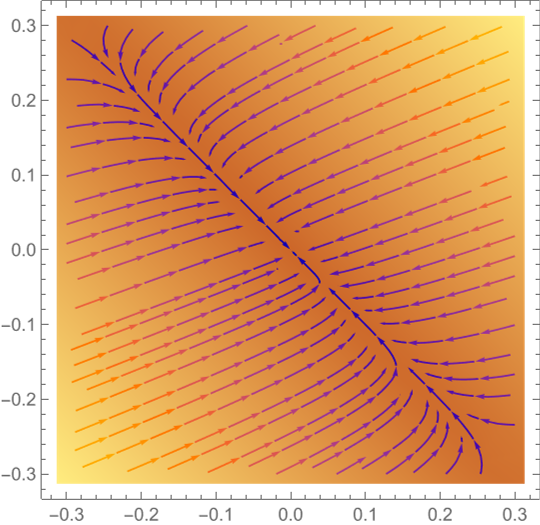
\includegraphics[width=\textwidth]{p1_1_1}
 		\caption{Фазовый портрет линейной системы}
 		\label{oldfazov}
 	\end{subfigure}
 	\qquad\qquad
 	\begin{subfigure}[H]{0.4\textwidth}
 		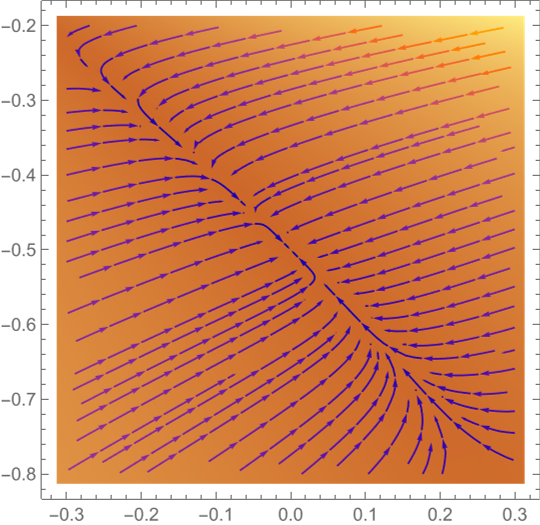
\includegraphics[width=\textwidth]{p1_1_2}
 		\caption{Фазовый портрет нелинейной системы}
 		\label{newfazov}
 	\end{subfigure}	
 	\\[0.2cm]
 	\caption{Асимптотически устойчивый узел}
 \end{figure}	
Заметим, что фазовые портреты похожи только в небольшой окрестности особой точки. Если мы удаляемся от особой точки, то нелинейные слагаемые начинают играть все большую роль, и фазовые портреты сильно различаются.
\begin{figure}[H]
	\centering
	\begin{subfigure}[H]{0.4\textwidth}
		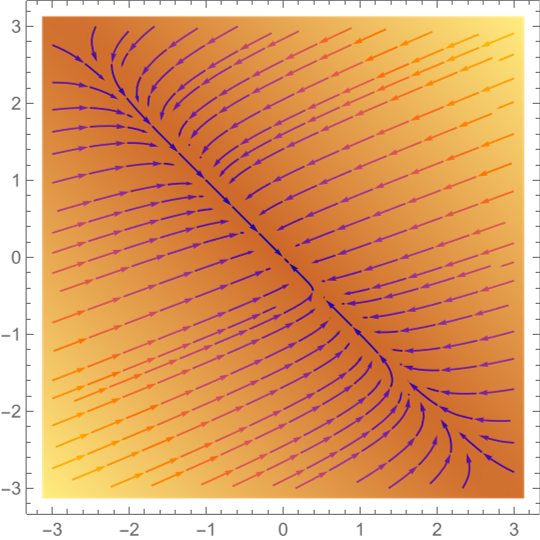
\includegraphics[width=\textwidth]{p1_2_1}
		\caption{Фазовый портрет линейной системы}
		\label{oldfazov}
	\end{subfigure}
	\qquad\qquad
	\begin{subfigure}[H]{0.4\textwidth}
		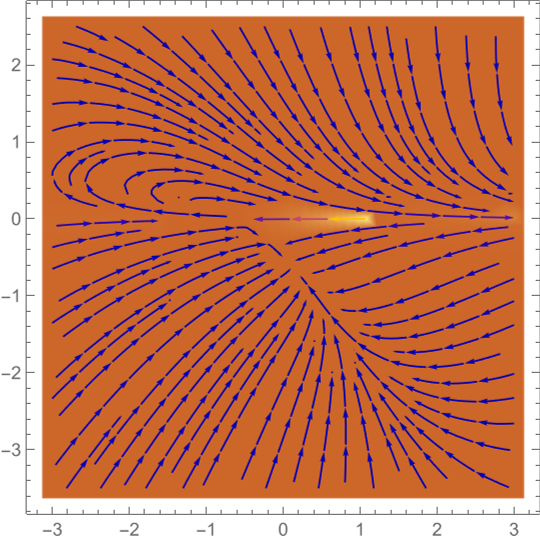
\includegraphics[width=\textwidth]{p1_2_2}
		\caption{Фазовый портрет нелинейной системы}
		\label{newfazov}
	\end{subfigure}	
	\\[0.2cm]
	\caption{Асимптотически устойчивый узел}
\end{figure}
\item  \textbf{Дикритический узел.} Параметры должны удовлетворять уравнению $4\alpha\beta=(\alpha+\beta+\frac{u\gamma\beta}{f_0})^2$. Пусть $\boldsymbol{f_0=23,\,\alpha=\beta=10,\,\gamma=0,\,u=0}$.

Нелинейная (\ref{system9}), линейная (\ref{system10}) системы и матрица Якоби (\ref{system11}), отвечающие этим параметрам:
\begin{gather*}
	\begin{cases}
		\dot \xi=-10\xi,\\
		\dot \eta=-10\eta,
	\end{cases}
	\qquad
	\begin{cases}
		\dot\xi=-10\xi,\\
		\dot \eta=-10\eta,
	\end{cases}
	\qquad
	\mathbb{J}=\begin{pmatrix}
		-10 & \phantom{-}0 \\
		\phantom{-}0 & -10
	\end{pmatrix}.
\end{gather*}
Видно, что линейная и нелинейная системы равны, значит фазовые портреты будут одинаковыми. Матрица Якоби диагональная --- собственные значения равны $\lambda_1=\lambda_2=-10$.
Т.к. собственные числа отрицательны, то фазовый портрет --- <<асимптотически устойчивый дикритический узел>>.

Жорданова форма матрицы $\mathbb{J}$ и матрица перехода имеют вид
\[
J=\begin{pmatrix}
	-10 & \phantom{-}0 \\
	\phantom{-}0 & -10
\end{pmatrix},
\quad
T=\begin{pmatrix}
	0 & 1 \\
	1 & 0
\end{pmatrix}.
\]
Система (\ref{system12}) имеет вид
\[
\begin{cases}
	\dot{\tilde{\xi}}=-10\tilde{\xi},\\
	\dot{\tilde{\eta}}=-10\tilde{\eta},
\end{cases}
\]
и фазовые траектории:
\[
\frac{d\tilde{\eta}}{d\tilde{\xi}}=\frac{\tilde\eta}{\tilde\xi}
\quad\Rightarrow\quad
\tilde{\eta}= C\tilde\xi\text{ --- пучок прямых}.
\]
\begin{figure}[H]
	\centering
	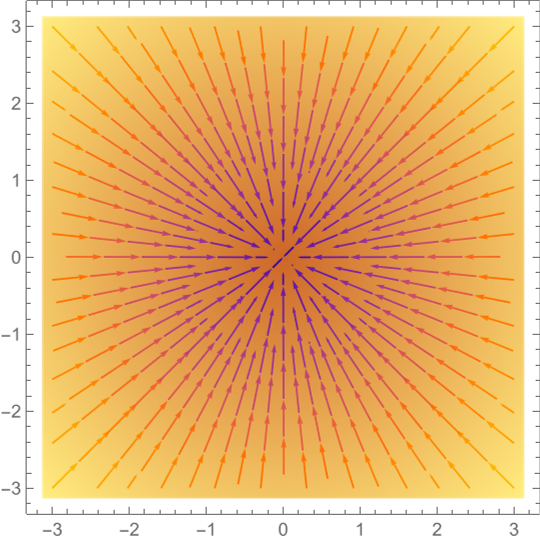
\includegraphics[width=7cm]{p2}
	\caption{Асимптотически устойчивый дикритический узел}
\end{figure}	
Все фазовые траектории (кроме особой точки) --- лучи прямых, каждая стремится к особой точке под собственным углом. Для нелинейной системы траектории не обязаны быть лучами прямых, но характеристическое свойство --- стремиться к особой точке под своим собственным углом --- у них сохраняется.
\item  \textbf{Вырожденный узел.} Параметры должны удовлетворять уравнению $4\alpha\beta=(\alpha+\beta+\frac{u\gamma\beta}{f_0})^2$. Пусть $\boldsymbol{f_0=3,\,\alpha=2,\,\beta=2,\,\gamma=0,\,u=1}$.

Нелинейная (\ref{system9}), линейная (\ref{system10}) системы и матрица Якоби (\ref{system11}), отвечающие этим параметрам:
\begin{gather*}
	\begin{cases}
		\dot \xi=2-2\xi+\sfrac{3}{\eta-\frac{3}{2}},\\
		\dot \eta=-2\eta,
	\end{cases}
	\qquad
	\begin{cases}
		\dot\xi=-2\xi-\sfrac{4}{3}\eta,\\
		\dot \eta=-2\eta,
	\end{cases}
	\qquad
	\mathbb{J}=\begin{pmatrix}
		-2 & -\sfrac{4}{3} \\
		\phantom{-}0 & -2
	\end{pmatrix}.
\end{gather*}
Матрица Якоби верхнетреугольная и значит ее собственные значения равны $\lambda_1=\lambda_2=-2$.
Т.к. собственные числа отрицательны, то фазовый портрет --- <<асимптотически устойчивый вырожденный узел>>.

Жорданова форма матрицы $\mathbb{J}$ и матрица перехода имеют вид
\[
J=\begin{pmatrix}
	-2 & \phantom{-}1 \\
	\phantom{-}0 & -2
\end{pmatrix},
\quad
T=\begin{pmatrix}
	1 & 0 \\
	0 & -\sfrac{3}{4}
\end{pmatrix}.
\]
Cистема (\ref{system12}) имеет вид
\[
\begin{cases}
	\dot{\tilde{\xi}}=-2\tilde{\xi}+\tilde{\eta},\\
	\dot{\tilde{\eta}}=-2\tilde{\eta}.
\end{cases}
\]
У матрицы есть единственный собственный вектор и все траектории такой системы, кроме особой точки, стремятся к особой точке, касаясь этого собственного вектора.
\begin{figure}[H]
	\centering
	\begin{subfigure}[H]{0.4\textwidth}
		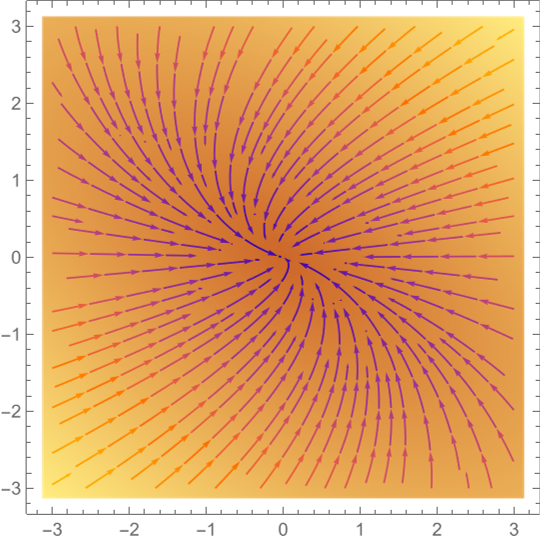
\includegraphics[width=\textwidth]{p3_1}
		\caption{Фазовый портрет линейной системы}
		\label{oldfazov}
	\end{subfigure}
	\qquad\qquad
	\begin{subfigure}[H]{0.4\textwidth}
		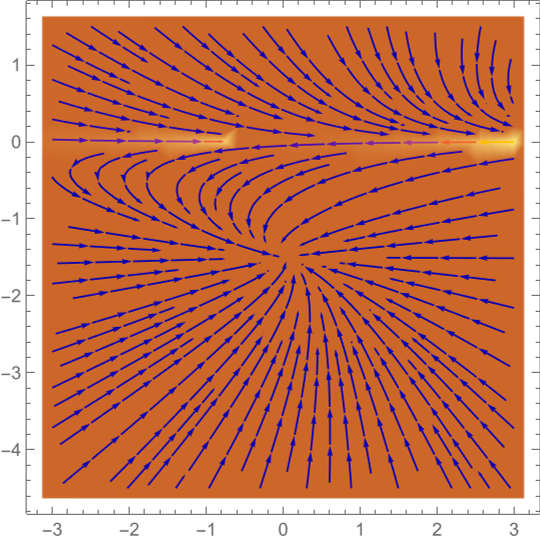
\includegraphics[width=\textwidth]{p3_2}
		\caption{Фазовый портрет нелинейной системы}
		\label{newfazov}
	\end{subfigure}	
	\\[0.2cm]
	\caption{Асимптотически устойчивый вырожденный узел}
\end{figure}	
\item \textbf{Фокус.} Параметры должны удовлетворять неравенству $4\alpha\beta>(\alpha+\beta+\frac{u\gamma\beta}{f_0})^2$.  Пусть $\boldsymbol{f_0=-1,\,\alpha=1,\,\beta=1,\,\gamma=-1,\,u=-1}$.

Нелинейная (\ref{system9}), линейная (\ref{system10}) системы и матрица Якоби (\ref{system11}), отвечающие этим параметрам:
\begin{gather*}
	\begin{cases}
		\dot \xi=-1-\xi-\sfrac{1+\xi}{1+\eta},\\
		\dot \eta=\xi-\eta,
	\end{cases}
	\qquad
	\begin{cases}
		\dot\xi=-\eta,\\
		\dot \eta=\xi-\eta,
	\end{cases}
	\qquad
	\mathbb{J}=\begin{pmatrix}
		0 & -1 \\
		1 & -1
	\end{pmatrix}.
\end{gather*}
Собственные значения равны
\[
\left[
\begin{array}{l}
	\lambda_1=\sfrac{-1+i\sqrt{3}}{2}, \\
	\lambda_2=\sfrac{-1-i\sqrt{3}}{2}.
\end{array}
\right.
\]
$\operatorname{Re}(\lambda_{1,2})<0$ --- асимптотически устойчивый фокус.

В отличие от узлов, траектории фокусов стремятся к особой точке, не касаясь какого-то направления, а совершая бесконечное число оборотов вокруг особой точки. Аналогичное утверждение справедливо и для соответствующей нелинейной системы.
\begin{figure}[H]
	\centering
	\begin{subfigure}[H]{0.4\textwidth}
		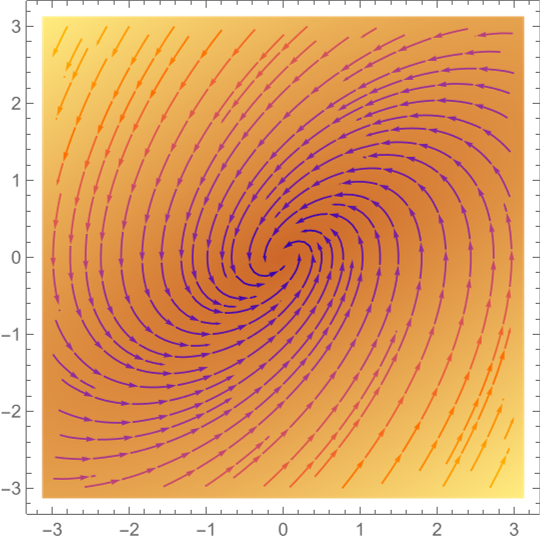
\includegraphics[width=\textwidth]{p4}
		\caption{Фазовый портрет линейной системы}
	\end{subfigure}
	\qquad\qquad
	\begin{subfigure}[H]{0.4\textwidth}
		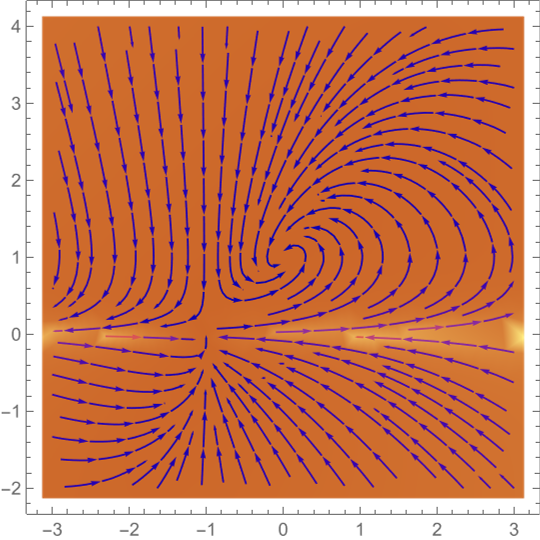
\includegraphics[width=\textwidth]{p44}
		\caption{Фазовый портрет нелинейной системы}
	\end{subfigure}	
	\\[0.2cm]
	\caption{Асимптотически устойчивый фокус}
\end{figure}	
\item \textbf{Седло.} Параметры должны удовлетворять неравенству $\alpha\beta<0$. Пусть $\boldsymbol{f_0=5,\,\alpha=3,\,\beta=-6,\,\gamma=3,\,u=0}$.

Нелинейная (\ref{system9}), линейная (\ref{system10}) системы и матрица Якоби (\ref{system11}), отвечающие этим параметрам:
\begin{gather*}
	\begin{cases}
		\dot \xi=-3\xi,\\
		\dot \eta=-3\xi+6\eta,
	\end{cases}
	\qquad
	\begin{cases}
		\dot\xi=-3\xi,\\
		\dot \eta=-3\xi+6\eta,
	\end{cases}
	\qquad
	\mathbb{J}=\begin{pmatrix}
		-3 & 0 \\
		-3 & 6
	\end{pmatrix}.
\end{gather*}
Собственные значения равны
\[
\left[
\begin{array}{l}
	\lambda_1=-3, \\
	\lambda_2=6.
\end{array}
\right.
\]
Жорданова форма матрицы $\mathbb{J}$ и матрица перехода имеют вид
\[
J=\begin{pmatrix}
	-3 & 0 \\
	\phantom{-}0 & 6
\end{pmatrix},
\quad
T=\begin{pmatrix}
	3 & 0 \\
	1 & 1
\end{pmatrix}.
\]
Cистема (\ref{system12}) имеет вид
\[
\begin{cases}
	\dot{\tilde{\xi}}=-3\tilde{\xi},\\
	\dot{\tilde{\eta}}=6\tilde{\eta}.
\end{cases}
\]
У седел фазовые кривые — ветви гипербол, кроме самой особой точки и четырёх прямолинейных лучей, называющихся \textbf{сепаратрисами}. Две сепаратрисы стремятся к седлу при $t\to+\infty$ вдоль собственного вектора с отрицательным собственным значениям (такие сепаратрисы называются входящими), две другие сепаратрисы стремятся к седлу при $t\to-\infty$ 
вдоль собственного вектора с положительным собственным значением (это исходящие сепаратрисы).
\begin{figure}[H]
	\centering
	\begin{subfigure}[H]{0.4\textwidth}
		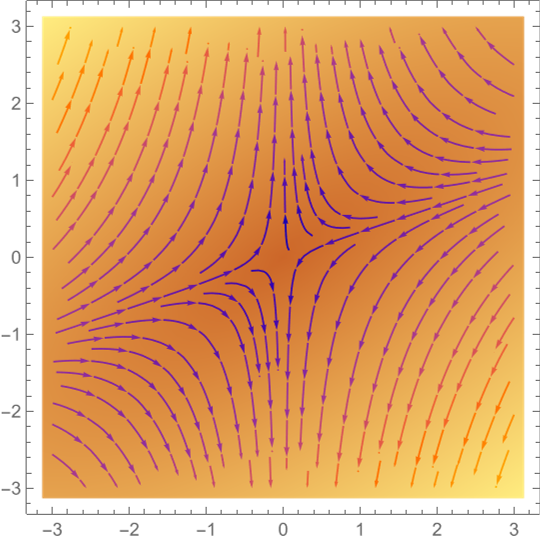
\includegraphics[width=\textwidth]{p5}
		\caption{Фазовый портрет линейной системы}
	\end{subfigure}
	\qquad\qquad
	\begin{subfigure}[H]{0.4\textwidth}
		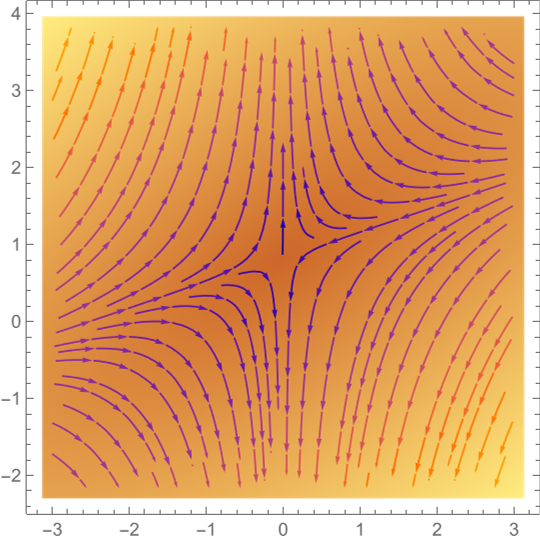
\includegraphics[width=\textwidth]{p55}
		\caption{Фазовый портрет нелинейной системы}
	\end{subfigure}	
	\\[0.2cm]
	\caption{Неустойчивое седло}
\end{figure}	
\item \textbf{Центр.} Во всех предыдущих примерах было справедливо неформальное утверждение «фазовый портрет вблизи нелинейной особой точки качественно похож на фазовый портрет линеаризации». Для центров это утверждение неверно. Фазовые кривые линейного центра обязательно замкнуты. Фазовые кривые соответствующей нелинейной особой точки могут быть спиралями.

Пусть $\boldsymbol{f_0=-2,\,\alpha=4,\,\beta=4,\,\gamma=2,\,u=1}$.

Нелинейная (\ref{system9}), линейная (\ref{system10}) системы и матрица Якоби (\ref{system11}), отвечающие этим параметрам:
\begin{gather*}
	\begin{cases}
		\dot \xi=5-5\xi+\sfrac{4\xi-2}{\eta+\frac{2}{5}},\\
		\dot \eta=-4\xi-5\eta,
	\end{cases}
	\qquad
	\begin{cases}
		\dot\xi=5\xi+\sfrac{25}{2}\eta,\\
		\dot \eta=-4\xi-5\eta,
	\end{cases}
	\qquad
	\mathbb{J}=\begin{pmatrix}
		\phantom{-}5 & \phantom{-}\sfrac{25}{2} \\
		-4 & -5
	\end{pmatrix}.
\end{gather*}
Собственные значения равны $\lambda_{1,2}=\pm5i.$\\
Жорданова форма матрицы $\mathbb{J}$ и матрица перехода имеют вид
\[
J=\begin{pmatrix}
	5i & \phantom{-}0 \\
	0 & -5i
\end{pmatrix},
\quad
T=\begin{pmatrix}
	\sfrac{-5-5i}{4} & \sfrac{-5+5i}{4} \\
	1 & 1
\end{pmatrix}.
\]
Cистема (\ref{system12}) имеет вид
\[
\begin{cases}
	\dot{\tilde{\xi}}=5i\tilde{\xi},\\
	\dot{\tilde{\eta}}=-5i\tilde{\eta}.
\end{cases}
\]
\begin{figure}[H]
	\centering
	\begin{subfigure}[H]{0.4\textwidth}
		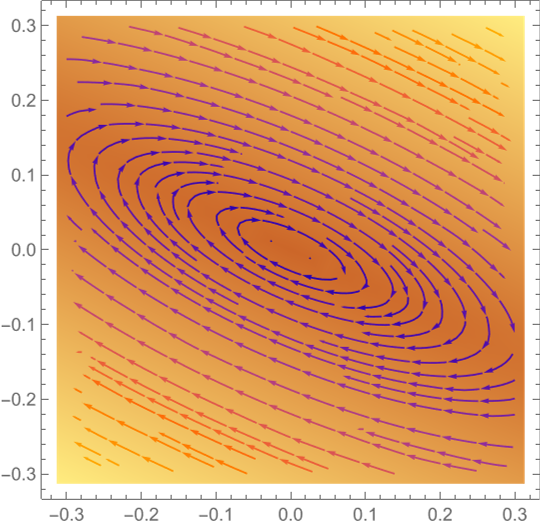
\includegraphics[width=\textwidth]{p6}
		\caption{Фазовый портрет линейной системы --- центр}
	\end{subfigure}
	\qquad\qquad
	\begin{subfigure}[H]{0.4\textwidth}
		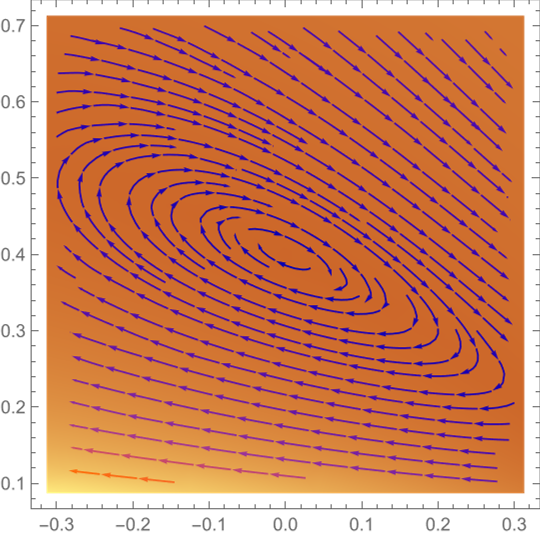
\includegraphics[width=\textwidth]{p66}
		\caption{Фазовый портрет нелинейной системы --- <<медленный>> фокус}
	\end{subfigure}	
	\\[0.2cm]
	\caption{Устойчивый центр}
\end{figure}	
	\item \textbf{Вырожденные случаи.} Это случаи, когда определитель матрицы $\mathbb{J}$ равен нулю. Вырожденные типы особых точек не имеют персональных названий.
\begin{enumerate}
	\item \textbf{Одно собственное значение равно нулю.} Пусть $\boldsymbol{f_0=390,\,\alpha=0,\,\beta=67,\,\gamma=22,\,u=13}$. 
	Из уравнения (\ref{xarakequation}) собственные числа равны
	\[
	\left[
	\begin{array}{l}
		\lambda_1=-\sfrac{1742}{15}, \\
		\lambda_2=0.
	\end{array}
	\right.
	\]
	Жорданова форма матрицы $A$ и матрица перехода имеют вид
	\[
	J=\begin{pmatrix}
		-\frac{1742}{15} & 0 \\
		\phantom{-}0 & 0
	\end{pmatrix},
	\quad
	T=\begin{pmatrix}
		\frac{67}{30} & -\frac{67}{22} \\
		1 & \phantom{-}1
	\end{pmatrix}.
	\]
	Система (\ref{system12}) имеет вид
	\[
	\begin{cases}
		\dot{\tilde{\xi}}=-\frac{1742}{15}\tilde{\xi},\\
		\dot{\tilde{\eta}}=0,
	\end{cases}
	\]
	и фазовые траектории оказываются прямыми:
	\[
	\frac{d\tilde{\eta}}{d\tilde{\xi}}=0
	\quad\Rightarrow\quad
	\tilde{\eta}\equiv 0.
	\]
	
	На рис.~\ref{newfazov} прямые параллельны оси абсцисс, т.е. прямой, отвечающей ненулевому собственному значению $\lambda_1$. Система параллельных прямых при линейном преобразовании плоскости переходит в систему параллельных прямых, поэтому и в исходной плоскости на рис.~\ref{oldfazov} мы получим систему прямых, параллельных той, которая отвечает ненулевому собственному значению. Отметим, что эта система прямых пересекает еще одну прямую отвечающую нулевому собственному значению $\lambda_2$ и состоящую целиком из особых точек.
	\begin{figure}[H]
		\centering
		\begin{subfigure}[H]{0.4\textwidth}
			\includegraphics[width=\textwidth]{j2\_1}
			\caption{Фазовый портрет в $(\xi,\eta)$}
			\label{oldfazov}
		\end{subfigure}
		\qquad\qquad
		\begin{subfigure}[H]{0.4\textwidth}
			\includegraphics[width=\textwidth]{j2\_2}
			\caption{Фазовый портрет в $(\tilde\xi,\tilde\eta)$}
			\label{newfazov}
		\end{subfigure}	
		\\[0.2cm]
		\caption{Фазовые портреты при $\alpha=0$}
	\end{figure}
	\item \textbf{Оба собственных значения равны нулю.} Пусть $\boldsymbol{f_0=-u\gamma=13\cdot 4,\,\alpha=0,\,\beta=5,\,\gamma=4,\,u=-13}$. Собственные значения равны $\lambda_{1,2}=0$.
	В этом случае возможны два варианта жордановой формы матрицы $\mathbb{J}$.
	Первый случай это
	\[
	J_1=\begin{pmatrix}
		0 & 1 \\
		0 & 0
	\end{pmatrix},
	\quad
	T_1=\begin{pmatrix}
		-\frac{5}{4} & -\frac{1}{4} \\
		\phantom{-}1 & \phantom{-}0
	\end{pmatrix},
	\]
	что соответствует системе дифференциальных уравнений
	\[
	\begin{cases}
		\dot{\tilde{\xi}}=\tilde{\eta},\\
		\dot{\tilde{\eta}}=0,
	\end{cases}
	\]
	для которой фазовые траектории оказываются прямыми $\tilde\eta =$ const, параллельными оси абсцисс (в отличие от предыдущего случая эта прямая отвечает нулевому собственному значению, т.е. состоит из особых точек). В исходной плоскости мы получим систему прямых, параллельных той, которая отвечает нулевому собственному значению.
	\begin{figure}[H]
		\centering
		\begin{subfigure}[H]{0.4\textwidth}
			\includegraphics[width=\textwidth]{j3\_1\_1}
			\caption{Фазовый портрет в $(\xi,\eta)$}
			\label{oldfazov2}
		\end{subfigure}
		\qquad\qquad
		\begin{subfigure}[H]{0.4\textwidth}
			\includegraphics[width=\textwidth]{j3\_1\_2}
			\caption{Фазовый портрет в $(\tilde\xi,\tilde\eta)$}
			\label{newfazov2}
		\end{subfigure}	
		\\[0.2cm]
		\caption{Фазовые портреты при $\lambda_{1,2}=0$}
	\end{figure}
	Второй случай --- когда жорданова форма матрицы $\mathbb{J}$ нулевая. В этом случае $\dot{\tilde\xi}=\dot{\tilde\eta}=0$,  и вся плоскость состоит из особых точек. Движения по фазовой плоскости нет, поэтому определять его направление уже нет необходимости.
\end{enumerate}	
	\end{enumerate}
	\subsection{Аналитическое решение системы}
	Для нахождения аналитического решения предположим, что $\gamma=f_0=0$. Тогда перепишем систему (\ref{system1}) в виде
	\begin{equation}
		\begin{cases}
			\dot v=u\beta-\alpha v, \\
			\dot m=-\beta m, \\
			v=v_0,\,t=0,\\
			m=m_0,\,t=0.
		\end{cases}
		\label{system7}
	\end{equation}
	Первое уравнение системы (\ref{system7}) --- уравнение с разделяющимися переменными. Найдем общий интеграл и частное решение, удовлетворяющее задаче Коши: 
	\[
	\frac{dv}{dt}=u\beta-\alpha v
	\;\Rightarrow\;
	\ln(|u\beta-\alpha v|)=-\alpha t+\ln|C|
	\;\Rightarrow\;
	v=\frac{u\beta-Ce^{-\alpha t}}{\alpha}.
	\]
	Решение задачи Коши:
	\[
	\begin{cases}
		v=\frac{u\beta-Ce^{-\alpha t}}{\alpha},\\
		v(0)=v_0,
	\end{cases}
	\;\Rightarrow\;
	C=u\beta-\alpha v_0
	\;\Rightarrow\;
	v=\frac{u\beta+(\alpha v_0-u\beta)e^{-\alpha t}}{\alpha}.
	\]
	Второе уравнение системы (\ref{system7}) --- уравнение с разделяющимися переменными. Найдем общий интеграл и частное решение удовлетворящее задаче Коши:
	\[
	\frac{dm}{m}=-\beta m
	\;\Rightarrow\;
	\ln|m|=-\beta t+\ln|C|
	\;\Rightarrow\;
	m=Ce^{-\beta t}.
	\]
	Решение задачи Коши:
	\[
	\begin{cases}
		m=Ce^{-\beta t},\\
		m(0)=m_0,
	\end{cases}
	\;\Rightarrow\;
	C=m_0
	\;\Rightarrow\;
	m=m_0e^{-\beta t}.
	\]
	Получим частное решение системы (\ref{system7})
	\[
	\begin{cases}
		v=\sfrac{u\beta+(\alpha v_0-u\beta)e^{-\alpha t}}{\alpha},\\
		m=m_0e^{-\beta t}.
	\end{cases}
	\]
	
	На рис.~\ref{graphic} представлены графики решений системы
	\begin{figure}[H]
		\centering
		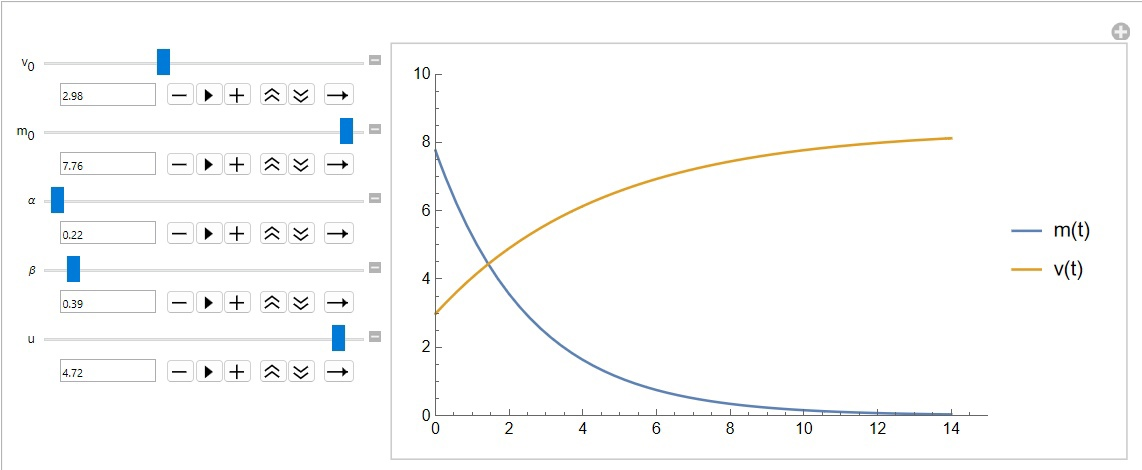
\includegraphics[width=\textwidth]{graphic}
		\caption{Решения системы (\ref{system7}) при $f_0=\gamma=0$}
		\label{graphic}
	\end{figure}	
	
	
	\section-{Заключение}
	Таким образом, в ходе выполнения курсовой работы качественно-аналитическим методом была исследована система ОДУ. Фазовые портреты нелинейных систем на плоскости можно исследовать, переходя к линеаризации. Для этого надо вычислить матрицу Якоби правой части системы в особой точке --- она и будет матрицей линеаризованной системы. Если линеаризация имеет особую точку типа узел, фокус или седло, фазовый портрет исходной (нелинейной) системы в окрестности особой точки похож на фазовый портрет линеаризации. Для центров это неверно: центры по линейным членам могут выглядеть как фокусы. К особым точкам с вырожденной матрицей линеаризации этот метод неприменим. 
	
	В работе также представлены рисунки фазовых портретов и графики аналитического решения системы, выполненные с использованием математического пакета Wolfram Mathematica.

	
	
	
	
	
	
	
	
	\newpage
	\begin{thebibliography}{1}
		\bibitem{Viki1} Динамическая система // Википедия. Свободная энциклопедия. URL:~https://ru.wikipedia.org/wiki/Динамическая\_система\\(дата обращения: 18.03.2022);
		\bibitem{Viki2} Линеаризация // Википедия. Свободная энциклопедия. URL:~https://ru.wikipedia.org/wiki/Линеаризация (дата обращения: 23.03.2022);
		\bibitem{Book1} Филиппов, А.Ф. Введение в теорию дифференциальных уравнений: Учебник, --- М.:Едиториал УРСС, 2004. --- 240 с.
		\bibitem{Book2} Агафонов С.А. Дифференциальные уравнения : учеб. для вузов / С.А. Агафонов, А.Д. Герман, Т.В. Муратова.-- Изд. 5-е стер. --- М.: Изд-во МГТУ им. Н.Э. Баумана, 2011. --- 347 с., [5] c.: ил. --- (Математика в техническом университете; вып. \RomanNumeralCaps{8});
		\bibitem{Book3} Демидович Б.П. Дифференциальные уравнения : учебное пособие для вузов / Б.П.~Демидович, В.П.~Моденов. --- 6-е изд., стер. --- Санкт-Петербург : Лань, 2022. --- 280 с.: ил. --- Текст : непосредственный.
		\bibitem{Book4} Петровский И.Г. Лекции по теории обыкновенных дифференциальных уравнений. --- М.: Наука, 1970. --- 280 с.
		
	\end{thebibliography}
	
	
\end{document}
